\documentclass{standalone}
\usepackage{tikz}
\usetikzlibrary{patterns, positioning}


\begin{document}
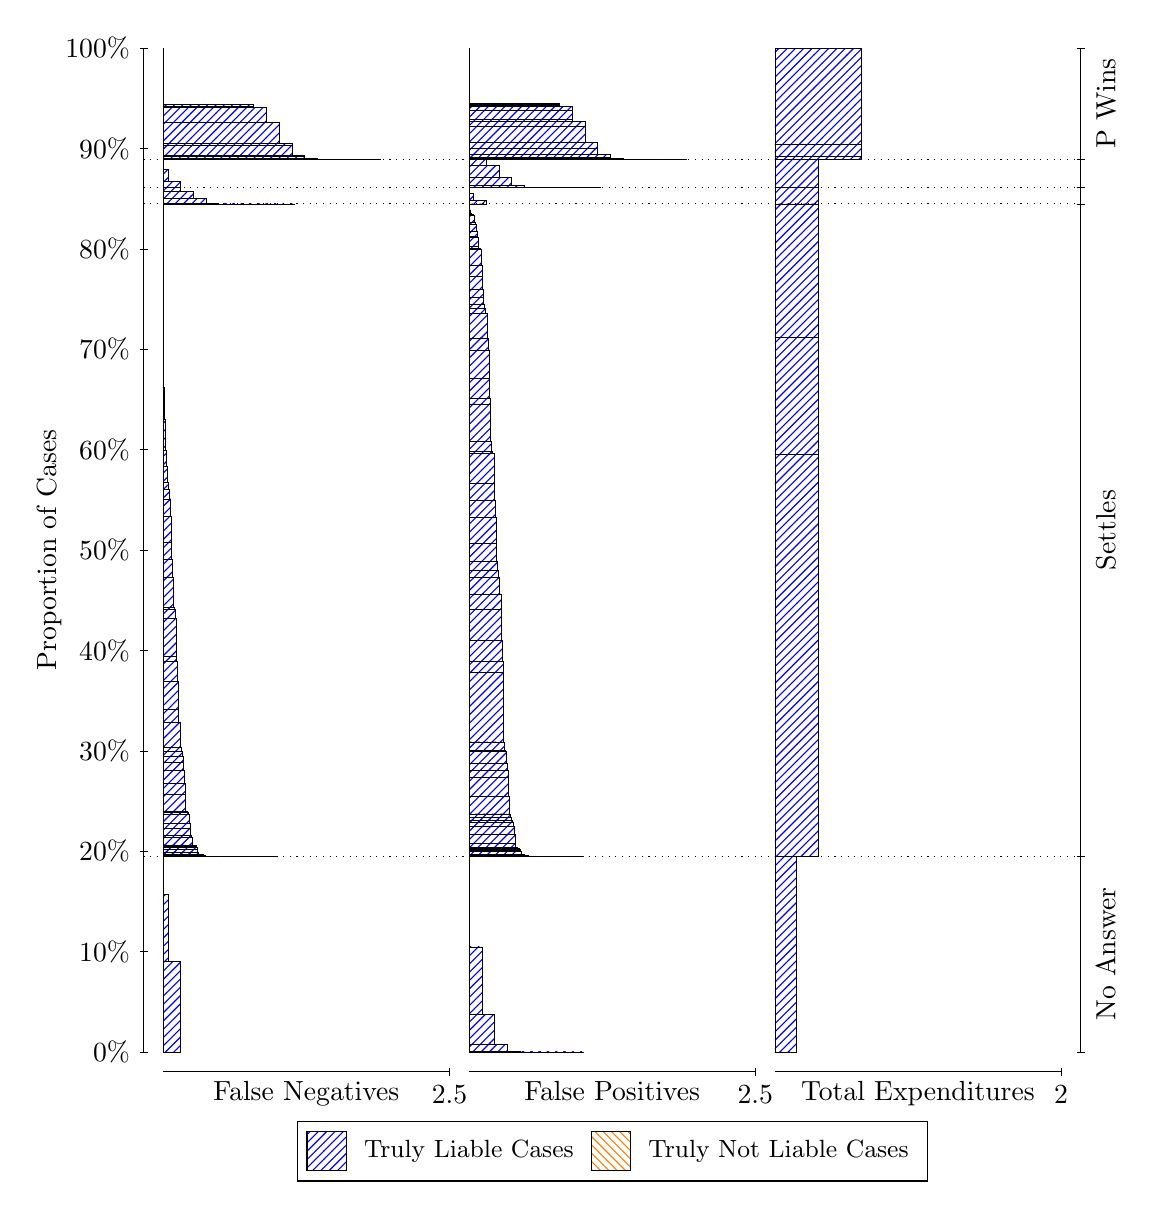
\begin{tikzpicture}
\draw[black, very thin] (1.5,1.75) -- (1.5,14.5);
\node[rotate=90, text=black, anchor=center] at (0.3, 8.125) {Proportion of Cases};
\draw[black, very thin] (1.45,1.75) -- (1.55,1.75);
\node[text=black, anchor=east] at (1.45, 1.75) {0\%};
\draw[black, very thin] (1.45,3.025) -- (1.55,3.025);
\node[text=black, anchor=east] at (1.45, 3.025) {10\%};
\draw[black, very thin] (1.45,4.3) -- (1.55,4.3);
\node[text=black, anchor=east] at (1.45, 4.3) {20\%};
\draw[black, very thin] (1.45,5.575) -- (1.55,5.575);
\node[text=black, anchor=east] at (1.45, 5.575) {30\%};
\draw[black, very thin] (1.45,6.85) -- (1.55,6.85);
\node[text=black, anchor=east] at (1.45, 6.85) {40\%};
\draw[black, very thin] (1.45,8.125) -- (1.55,8.125);
\node[text=black, anchor=east] at (1.45, 8.125) {50\%};
\draw[black, very thin] (1.45,9.4) -- (1.55,9.4);
\node[text=black, anchor=east] at (1.45, 9.4) {60\%};
\draw[black, very thin] (1.45,10.675) -- (1.55,10.675);
\node[text=black, anchor=east] at (1.45, 10.675) {70\%};
\draw[black, very thin] (1.45,11.95) -- (1.55,11.95);
\node[text=black, anchor=east] at (1.45, 11.95) {80\%};
\draw[black, very thin] (1.45,13.225) -- (1.55,13.225);
\node[text=black, anchor=east] at (1.45, 13.225) {90\%};
\draw[black, very thin] (1.45,14.5) -- (1.55,14.5);
\node[text=black, anchor=east] at (1.45, 14.5) {100\%};

\draw[black, very thin] (13.4,1.75) -- (13.4,14.5);
\draw[black, very thin] (13.35,1.75) -- (13.45,1.75);
\node[anchor=west] at (13.35, 1.75) {};
\draw[black, very thin] (13.35,4.2363) -- (13.45,4.2363);
\node[anchor=west] at (13.35, 4.2363) {};
\draw[black, very thin] (13.35,12.521) -- (13.45,12.521);
\node[anchor=west] at (13.35, 12.521) {};
\draw[black, very thin] (13.35,12.727) -- (13.45,12.727);
\node[anchor=west] at (13.35, 12.727) {};
\draw[black, very thin] (13.35,13.085) -- (13.45,13.085);
\node[anchor=west] at (13.35, 13.085) {};
\draw[black, very thin] (13.35,14.5) -- (13.45,14.5);
\node[anchor=west] at (13.35, 14.5) {};

\draw[black, very thin, pattern color=blue, pattern=north east lines] (1.75,1.75) rectangle (1.968,2.9018);
\draw[black, very thin, pattern color=blue, pattern=north east lines] (1.75,2.9018) rectangle (1.8065,3.7553);
\draw[black, very thin, pattern color=orange, pattern=north west lines] (1.75,3.7553) rectangle (1.75,3.7553);
\draw[black, very thin, pattern color=blue, pattern=north east lines] (1.75,3.7553) rectangle (1.75,4.2363);
\draw[black, very thin, pattern color=blue, pattern=north east lines] (1.75,4.2363) rectangle (3.2033,4.2363);
\draw[black, very thin, pattern color=blue, pattern=north east lines] (1.75,4.2363) rectangle (3.1307,4.2363);
\draw[black, very thin, pattern color=blue, pattern=north east lines] (1.75,4.2363) rectangle (3.058,4.2363);
\draw[black, very thin, pattern color=blue, pattern=north east lines] (1.75,4.2363) rectangle (3.0419,4.2363);
\draw[black, very thin, pattern color=blue, pattern=north east lines] (1.75,4.2363) rectangle (2.9853,4.2363);
\draw[black, very thin, pattern color=blue, pattern=north east lines] (1.75,4.2363) rectangle (2.9692,4.2363);
\draw[black, very thin, pattern color=blue, pattern=north east lines] (1.75,4.2363) rectangle (2.9127,4.2363);
\draw[black, very thin, pattern color=blue, pattern=north east lines] (1.75,4.2363) rectangle (2.8965,4.2363);
\draw[black, very thin, pattern color=blue, pattern=north east lines] (1.75,4.2363) rectangle (2.8804,4.2363);
\draw[black, very thin, pattern color=blue, pattern=north east lines] (1.75,4.2363) rectangle (2.84,4.2363);
\draw[black, very thin, pattern color=blue, pattern=north east lines] (1.75,4.2363) rectangle (2.8239,4.2363);
\draw[black, very thin, pattern color=blue, pattern=north east lines] (1.75,4.2363) rectangle (2.8077,4.2363);
\draw[black, very thin, pattern color=blue, pattern=north east lines] (1.75,4.2363) rectangle (2.7673,4.2363);
\draw[black, very thin, pattern color=blue, pattern=north east lines] (1.75,4.2363) rectangle (2.7512,4.2363);
\draw[black, very thin, pattern color=blue, pattern=north east lines] (1.75,4.2363) rectangle (2.735,4.2363);
\draw[black, very thin, pattern color=blue, pattern=north east lines] (1.75,4.2363) rectangle (2.7189,4.2363);
\draw[black, very thin, pattern color=blue, pattern=north east lines] (1.75,4.2363) rectangle (2.6947,4.2363);
\draw[black, very thin, pattern color=blue, pattern=north east lines] (1.75,4.2363) rectangle (2.6785,4.2363);
\draw[black, very thin, pattern color=blue, pattern=north east lines] (1.75,4.2363) rectangle (2.6624,4.2363);
\draw[black, very thin, pattern color=blue, pattern=north east lines] (1.75,4.2363) rectangle (2.6462,4.2363);
\draw[black, very thin, pattern color=blue, pattern=north east lines] (1.75,4.2363) rectangle (2.622,4.2363);
\draw[black, very thin, pattern color=blue, pattern=north east lines] (1.75,4.2363) rectangle (2.6059,4.2363);
\draw[black, very thin, pattern color=blue, pattern=north east lines] (1.75,4.2363) rectangle (2.5897,4.2363);
\draw[black, very thin, pattern color=blue, pattern=north east lines] (1.75,4.2363) rectangle (2.5736,4.2363);
\draw[black, very thin, pattern color=blue, pattern=north east lines] (1.75,4.2363) rectangle (2.5574,4.2363);
\draw[black, very thin, pattern color=blue, pattern=north east lines] (1.75,4.2363) rectangle (2.5493,4.2363);
\draw[black, very thin, pattern color=blue, pattern=north east lines] (1.75,4.2363) rectangle (2.5332,4.2363);
\draw[black, very thin, pattern color=blue, pattern=north east lines] (1.75,4.2363) rectangle (2.517,4.2363);
\draw[black, very thin, pattern color=blue, pattern=north east lines] (1.75,4.2363) rectangle (2.5009,4.2363);
\draw[black, very thin, pattern color=blue, pattern=north east lines] (1.75,4.2363) rectangle (2.4847,4.2363);
\draw[black, very thin, pattern color=blue, pattern=north east lines] (1.75,4.2363) rectangle (2.4767,4.2363);
\draw[black, very thin, pattern color=blue, pattern=north east lines] (1.75,4.2363) rectangle (2.4605,4.2363);
\draw[black, very thin, pattern color=blue, pattern=north east lines] (1.75,4.2363) rectangle (2.4444,4.2364);
\draw[black, very thin, pattern color=blue, pattern=north east lines] (1.75,4.2364) rectangle (2.4282,4.2364);
\draw[black, very thin, pattern color=blue, pattern=north east lines] (1.75,4.2364) rectangle (2.4121,4.2364);
\draw[black, very thin, pattern color=blue, pattern=north east lines] (1.75,4.2364) rectangle (2.404,4.2364);
\draw[black, very thin, pattern color=blue, pattern=north east lines] (1.75,4.2364) rectangle (2.3959,4.2366);
\draw[black, very thin, pattern color=blue, pattern=north east lines] (1.75,4.2366) rectangle (2.3879,4.2366);
\draw[black, very thin, pattern color=blue, pattern=north east lines] (1.75,4.2366) rectangle (2.3717,4.2366);
\draw[black, very thin, pattern color=blue, pattern=north east lines] (1.75,4.2366) rectangle (2.3556,4.2371);
\draw[black, very thin, pattern color=blue, pattern=north east lines] (1.75,4.2371) rectangle (2.3394,4.2385);
\draw[black, very thin, pattern color=blue, pattern=north east lines] (1.75,4.2385) rectangle (2.3313,4.2387);
\draw[black, very thin, pattern color=blue, pattern=north east lines] (1.75,4.2387) rectangle (2.3233,4.2389);
\draw[black, very thin, pattern color=blue, pattern=north east lines] (1.75,4.2389) rectangle (2.3152,4.239);
\draw[black, very thin, pattern color=blue, pattern=north east lines] (1.75,4.239) rectangle (2.299,4.2391);
\draw[black, very thin, pattern color=blue, pattern=north east lines] (1.75,4.2391) rectangle (2.2829,4.2443);
\draw[black, very thin, pattern color=blue, pattern=north east lines] (1.75,4.2443) rectangle (2.2667,4.245);
\draw[black, very thin, pattern color=blue, pattern=north east lines] (1.75,4.245) rectangle (2.2587,4.2523);
\draw[black, very thin, pattern color=blue, pattern=north east lines] (1.75,4.2523) rectangle (2.2506,4.2554);
\draw[black, very thin, pattern color=blue, pattern=north east lines] (1.75,4.2554) rectangle (2.2425,4.2555);
\draw[black, very thin, pattern color=blue, pattern=north east lines] (1.75,4.2555) rectangle (2.2344,4.2646);
\draw[black, very thin, pattern color=blue, pattern=north east lines] (1.75,4.2646) rectangle (2.2264,4.2655);
\draw[black, very thin, pattern color=blue, pattern=north east lines] (1.75,4.2655) rectangle (2.2102,4.2661);
\draw[black, very thin, pattern color=blue, pattern=north east lines] (1.75,4.2661) rectangle (2.1941,4.2907);
\draw[black, very thin, pattern color=blue, pattern=north east lines] (1.75,4.2907) rectangle (2.186,4.3204);
\draw[black, very thin, pattern color=blue, pattern=north east lines] (1.75,4.3204) rectangle (2.1779,4.3527);
\draw[black, very thin, pattern color=blue, pattern=north east lines] (1.75,4.3527) rectangle (2.1699,4.3599);
\draw[black, very thin, pattern color=blue, pattern=north east lines] (1.75,4.3599) rectangle (2.1618,4.3688);
\draw[black, very thin, pattern color=blue, pattern=north east lines] (1.75,4.3688) rectangle (2.1537,4.3742);
\draw[black, very thin, pattern color=blue, pattern=north east lines] (1.75,4.3742) rectangle (2.1376,4.3809);
\draw[black, very thin, pattern color=blue, pattern=north east lines] (1.75,4.3809) rectangle (2.1214,4.4757);
\draw[black, very thin, pattern color=blue, pattern=north east lines] (1.75,4.4757) rectangle (2.1053,4.5001);
\draw[black, very thin, pattern color=blue, pattern=north east lines] (1.75,4.5001) rectangle (2.0972,4.5868);
\draw[black, very thin, pattern color=blue, pattern=north east lines] (1.75,4.5868) rectangle (2.0891,4.649);
\draw[black, very thin, pattern color=blue, pattern=north east lines] (1.75,4.649) rectangle (2.081,4.6552);
\draw[black, very thin, pattern color=blue, pattern=north east lines] (1.75,4.6552) rectangle (2.073,4.7739);
\draw[black, very thin, pattern color=blue, pattern=north east lines] (1.75,4.7739) rectangle (2.0649,4.7983);
\draw[black, very thin, pattern color=blue, pattern=north east lines] (1.75,4.7983) rectangle (2.0487,4.8073);
\draw[black, very thin, pattern color=blue, pattern=north east lines] (1.75,4.8073) rectangle (2.0326,5.02);
\draw[black, very thin, pattern color=blue, pattern=north east lines] (1.75,5.02) rectangle (2.0245,5.16);
\draw[black, very thin, pattern color=blue, pattern=north east lines] (1.75,5.16) rectangle (2.0164,5.327);
\draw[black, very thin, pattern color=blue, pattern=north east lines] (1.75,5.327) rectangle (2.0084,5.4236);
\draw[black, very thin, pattern color=blue, pattern=north east lines] (1.75,5.4236) rectangle (2.0003,5.5097);
\draw[black, very thin, pattern color=blue, pattern=north east lines] (1.75,5.5097) rectangle (1.9922,5.5675);
\draw[black, very thin, pattern color=blue, pattern=north east lines] (1.75,5.5675) rectangle (1.9761,5.6242);
\draw[black, very thin, pattern color=blue, pattern=north east lines] (1.75,5.6242) rectangle (1.9599,5.9394);
\draw[black, very thin, pattern color=blue, pattern=north east lines] (1.75,5.9394) rectangle (1.9438,6.0992);
\draw[black, very thin, pattern color=blue, pattern=north east lines] (1.75,6.0992) rectangle (1.9357,6.4537);
\draw[black, very thin, pattern color=blue, pattern=north east lines] (1.75,6.4537) rectangle (1.9276,6.7109);
\draw[black, very thin, pattern color=blue, pattern=north east lines] (1.75,6.7109) rectangle (1.9196,6.7782);
\draw[black, very thin, pattern color=blue, pattern=north east lines] (1.75,6.7782) rectangle (1.9115,7.2541);
\draw[black, very thin, pattern color=blue, pattern=north east lines] (1.75,7.2541) rectangle (1.9034,7.3782);
\draw[black, very thin, pattern color=blue, pattern=north east lines] (1.75,7.3782) rectangle (1.8873,7.4026);
\draw[black, very thin, pattern color=blue, pattern=north east lines] (1.75,7.4026) rectangle (1.8711,7.7796);
\draw[black, very thin, pattern color=blue, pattern=north east lines] (1.75,7.7796) rectangle (1.863,8.004);
\draw[black, very thin, pattern color=blue, pattern=north east lines] (1.75,8.004) rectangle (1.855,8.222);
\draw[black, very thin, pattern color=blue, pattern=north east lines] (1.75,8.222) rectangle (1.8469,8.5508);
\draw[black, very thin, pattern color=blue, pattern=north east lines] (1.75,8.5508) rectangle (1.8388,8.773);
\draw[black, very thin, pattern color=blue, pattern=north east lines] (1.75,8.773) rectangle (1.8307,8.8899);
\draw[black, very thin, pattern color=blue, pattern=north east lines] (1.75,8.8899) rectangle (1.8146,8.9849);
\draw[black, very thin, pattern color=blue, pattern=north east lines] (1.75,8.9849) rectangle (1.7984,9.1899);
\draw[black, very thin, pattern color=blue, pattern=north east lines] (1.75,9.1899) rectangle (1.7823,9.3871);
\draw[black, very thin, pattern color=blue, pattern=north east lines] (1.75,9.3871) rectangle (1.7742,9.7801);
\draw[black, very thin, pattern color=blue, pattern=north east lines] (1.75,9.7801) rectangle (1.7661,10.051);
\draw[black, very thin, pattern color=blue, pattern=north east lines] (1.75,10.051) rectangle (1.7581,10.189);
\draw[black, very thin, pattern color=orange, pattern=north west lines] (1.75,10.189) rectangle (1.75,10.189);
\draw[black, very thin, pattern color=blue, pattern=north east lines] (1.75,10.189) rectangle (1.75,12.521);
\draw[black, very thin, pattern color=blue, pattern=north east lines] (1.75,12.521) rectangle (3.4213,12.521);
\draw[black, very thin, pattern color=blue, pattern=north east lines] (1.75,12.521) rectangle (3.2599,12.521);
\draw[black, very thin, pattern color=blue, pattern=north east lines] (1.75,12.521) rectangle (3.0984,12.521);
\draw[black, very thin, pattern color=blue, pattern=north east lines] (1.75,12.521) rectangle (2.9369,12.521);
\draw[black, very thin, pattern color=blue, pattern=north east lines] (1.75,12.521) rectangle (2.7754,12.521);
\draw[black, very thin, pattern color=blue, pattern=north east lines] (1.75,12.521) rectangle (2.6139,12.522);
\draw[black, very thin, pattern color=blue, pattern=north east lines] (1.75,12.522) rectangle (2.4524,12.53);
\draw[black, very thin, pattern color=blue, pattern=north east lines] (1.75,12.53) rectangle (2.291,12.592);
\draw[black, very thin, pattern color=blue, pattern=north east lines] (1.75,12.592) rectangle (2.1295,12.684);
\draw[black, very thin, pattern color=blue, pattern=north east lines] (1.75,12.684) rectangle (1.968,12.727);
\draw[black, very thin, pattern color=orange, pattern=north west lines] (1.75,12.727) rectangle (1.75,12.727);
\draw[black, very thin, pattern color=blue, pattern=north east lines] (1.75,12.727) rectangle (1.968,12.806);
\draw[black, very thin, pattern color=blue, pattern=north east lines] (1.75,12.806) rectangle (1.8065,12.957);
\draw[black, very thin, pattern color=orange, pattern=north west lines] (1.75,12.957) rectangle (1.75,12.957);
\draw[black, very thin, pattern color=blue, pattern=north east lines] (1.75,12.957) rectangle (1.75,13.085);
\draw[black, very thin, pattern color=blue, pattern=north east lines] (1.75,13.085) rectangle (4.5113,13.085);
\draw[black, very thin, pattern color=blue, pattern=north east lines] (1.75,13.085) rectangle (4.3499,13.085);
\draw[black, very thin, pattern color=blue, pattern=north east lines] (1.75,13.085) rectangle (4.1884,13.085);
\draw[black, very thin, pattern color=blue, pattern=north east lines] (1.75,13.085) rectangle (4.0269,13.085);
\draw[black, very thin, pattern color=blue, pattern=north east lines] (1.75,13.085) rectangle (4.0269,13.085);
\draw[black, very thin, pattern color=blue, pattern=north east lines] (1.75,13.085) rectangle (3.8654,13.086);
\draw[black, very thin, pattern color=blue, pattern=north east lines] (1.75,13.086) rectangle (3.8654,13.086);
\draw[black, very thin, pattern color=blue, pattern=north east lines] (1.75,13.086) rectangle (3.7039,13.087);
\draw[black, very thin, pattern color=blue, pattern=north east lines] (1.75,13.087) rectangle (3.7039,13.095);
\draw[black, very thin, pattern color=blue, pattern=north east lines] (1.75,13.095) rectangle (3.5424,13.119);
\draw[black, very thin, pattern color=blue, pattern=north east lines] (1.75,13.119) rectangle (3.5424,13.14);
\draw[black, very thin, pattern color=blue, pattern=north east lines] (1.75,13.14) rectangle (3.381,13.267);
\draw[black, very thin, pattern color=blue, pattern=north east lines] (1.75,13.267) rectangle (3.381,13.29);
\draw[black, very thin, pattern color=blue, pattern=north east lines] (1.75,13.29) rectangle (3.2195,13.558);
\draw[black, very thin, pattern color=blue, pattern=north east lines] (1.75,13.558) rectangle (3.058,13.75);
\draw[black, very thin, pattern color=blue, pattern=north east lines] (1.75,13.75) rectangle (2.8965,13.76);
\draw[black, very thin, pattern color=blue, pattern=north east lines] (1.75,13.76) rectangle (2.8965,13.785);
\draw[black, very thin, pattern color=blue, pattern=north east lines] (1.75,13.785) rectangle (2.735,13.785);
\draw[black, very thin, pattern color=blue, pattern=north east lines] (1.75,13.785) rectangle (2.735,13.786);
\draw[black, very thin, pattern color=blue, pattern=north east lines] (1.75,13.786) rectangle (2.735,13.786);
\draw[black, very thin, pattern color=blue, pattern=north east lines] (1.75,13.786) rectangle (2.5736,13.786);
\draw[black, very thin, pattern color=blue, pattern=north east lines] (1.75,13.786) rectangle (2.5736,13.786);
\draw[black, very thin, pattern color=blue, pattern=north east lines] (1.75,13.786) rectangle (2.4444,13.786);
\draw[black, very thin, pattern color=blue, pattern=north east lines] (1.75,13.786) rectangle (2.4121,13.786);
\draw[black, very thin, pattern color=blue, pattern=north east lines] (1.75,13.786) rectangle (2.4121,13.786);
\draw[black, very thin, pattern color=blue, pattern=north east lines] (1.75,13.786) rectangle (2.2829,13.786);
\draw[black, very thin, pattern color=blue, pattern=north east lines] (1.75,13.786) rectangle (2.2506,13.786);
\draw[black, very thin, pattern color=blue, pattern=north east lines] (1.75,13.786) rectangle (2.2506,13.786);
\draw[black, very thin, pattern color=blue, pattern=north east lines] (1.75,13.786) rectangle (2.1214,13.786);
\draw[black, very thin, pattern color=blue, pattern=north east lines] (1.75,13.786) rectangle (2.1214,13.786);
\draw[black, very thin, pattern color=blue, pattern=north east lines] (1.75,13.786) rectangle (2.0891,13.786);
\draw[black, very thin, pattern color=blue, pattern=north east lines] (1.75,13.786) rectangle (2.0891,13.786);
\draw[black, very thin, pattern color=blue, pattern=north east lines] (1.75,13.786) rectangle (1.9599,13.786);
\draw[black, very thin, pattern color=blue, pattern=north east lines] (1.75,13.786) rectangle (1.9599,13.786);
\draw[black, very thin, pattern color=blue, pattern=north east lines] (1.75,13.786) rectangle (1.9276,13.786);
\draw[black, very thin, pattern color=blue, pattern=north east lines] (1.75,13.786) rectangle (1.7984,13.786);
\draw[black, very thin, pattern color=blue, pattern=north east lines] (1.75,13.786) rectangle (1.7984,13.786);
\draw[black, very thin, pattern color=blue, pattern=north east lines] (1.75,13.786) rectangle (1.7984,13.786);
\draw[black, very thin, pattern color=orange, pattern=north west lines] (1.75,13.786) rectangle (1.75,13.786);
\draw[black, very thin, pattern color=blue, pattern=north east lines] (1.75,13.786) rectangle (1.75,14.5);
\draw[black, very thin, pattern color=orange, pattern=north west lines] (5.6333,1.75) rectangle (7.0867,1.75);
\draw[black, very thin, pattern color=blue, pattern=north east lines] (5.6333,1.75) rectangle (7.0867,1.75);
\draw[black, very thin, pattern color=blue, pattern=north east lines] (5.6333,1.75) rectangle (6.9252,1.75);
\draw[black, very thin, pattern color=blue, pattern=north east lines] (5.6333,1.75) rectangle (6.7637,1.75);
\draw[black, very thin, pattern color=blue, pattern=north east lines] (5.6333,1.75) rectangle (6.6022,1.75);
\draw[black, very thin, pattern color=blue, pattern=north east lines] (5.6333,1.75) rectangle (6.4407,1.7503);
\draw[black, very thin, pattern color=blue, pattern=north east lines] (5.6333,1.7503) rectangle (6.2793,1.7582);
\draw[black, very thin, pattern color=blue, pattern=north east lines] (5.6333,1.7582) rectangle (6.1178,1.8431);
\draw[black, very thin, pattern color=blue, pattern=north east lines] (5.6333,1.8431) rectangle (5.9563,2.231);
\draw[black, very thin, pattern color=blue, pattern=north east lines] (5.6333,2.231) rectangle (5.7948,3.0845);
\draw[black, very thin, pattern color=blue, pattern=north east lines] (5.6333,3.0845) rectangle (5.6333,4.2363);
\draw[black, very thin, pattern color=orange, pattern=north west lines] (5.6333,4.2363) rectangle (7.0867,4.2363);
\draw[black, very thin, pattern color=blue, pattern=north east lines] (5.6333,4.2363) rectangle (7.0867,4.2363);
\draw[black, very thin, pattern color=orange, pattern=north west lines] (5.6333,4.2363) rectangle (7.014,4.2363);
\draw[black, very thin, pattern color=blue, pattern=north east lines] (5.6333,4.2363) rectangle (7.014,4.2363);
\draw[black, very thin, pattern color=orange, pattern=north west lines] (5.6333,4.2363) rectangle (6.9413,4.2363);
\draw[black, very thin, pattern color=blue, pattern=north east lines] (5.6333,4.2363) rectangle (6.9413,4.2363);
\draw[black, very thin, pattern color=blue, pattern=north east lines] (5.6333,4.2363) rectangle (6.9252,4.2363);
\draw[black, very thin, pattern color=orange, pattern=north west lines] (5.6333,4.2363) rectangle (6.8687,4.2363);
\draw[black, very thin, pattern color=blue, pattern=north east lines] (5.6333,4.2363) rectangle (6.8687,4.2363);
\draw[black, very thin, pattern color=blue, pattern=north east lines] (5.6333,4.2363) rectangle (6.8525,4.2363);
\draw[black, very thin, pattern color=orange, pattern=north west lines] (5.6333,4.2363) rectangle (6.796,4.2363);
\draw[black, very thin, pattern color=blue, pattern=north east lines] (5.6333,4.2363) rectangle (6.796,4.2363);
\draw[black, very thin, pattern color=blue, pattern=north east lines] (5.6333,4.2363) rectangle (6.7799,4.2363);
\draw[black, very thin, pattern color=blue, pattern=north east lines] (5.6333,4.2363) rectangle (6.7637,4.2363);
\draw[black, very thin, pattern color=orange, pattern=north west lines] (5.6333,4.2363) rectangle (6.7233,4.2363);
\draw[black, very thin, pattern color=blue, pattern=north east lines] (5.6333,4.2363) rectangle (6.7233,4.2363);
\draw[black, very thin, pattern color=blue, pattern=north east lines] (5.6333,4.2363) rectangle (6.7072,4.2363);
\draw[black, very thin, pattern color=blue, pattern=north east lines] (5.6333,4.2363) rectangle (6.691,4.2363);
\draw[black, very thin, pattern color=orange, pattern=north west lines] (5.6333,4.2363) rectangle (6.6507,4.2363);
\draw[black, very thin, pattern color=blue, pattern=north east lines] (5.6333,4.2363) rectangle (6.6507,4.2363);
\draw[black, very thin, pattern color=blue, pattern=north east lines] (5.6333,4.2363) rectangle (6.6345,4.2363);
\draw[black, very thin, pattern color=blue, pattern=north east lines] (5.6333,4.2363) rectangle (6.6184,4.2363);
\draw[black, very thin, pattern color=blue, pattern=north east lines] (5.6333,4.2363) rectangle (6.6022,4.2363);
\draw[black, very thin, pattern color=orange, pattern=north west lines] (5.6333,4.2363) rectangle (6.578,4.2363);
\draw[black, very thin, pattern color=blue, pattern=north east lines] (5.6333,4.2363) rectangle (6.578,4.2363);
\draw[black, very thin, pattern color=blue, pattern=north east lines] (5.6333,4.2363) rectangle (6.5619,4.2363);
\draw[black, very thin, pattern color=blue, pattern=north east lines] (5.6333,4.2363) rectangle (6.5457,4.2364);
\draw[black, very thin, pattern color=blue, pattern=north east lines] (5.6333,4.2364) rectangle (6.5296,4.2365);
\draw[black, very thin, pattern color=orange, pattern=north west lines] (5.6333,4.2365) rectangle (6.5053,4.2365);
\draw[black, very thin, pattern color=blue, pattern=north east lines] (5.6333,4.2365) rectangle (6.5053,4.2365);
\draw[black, very thin, pattern color=blue, pattern=north east lines] (5.6333,4.2365) rectangle (6.4892,4.2365);
\draw[black, very thin, pattern color=blue, pattern=north east lines] (5.6333,4.2365) rectangle (6.473,4.2365);
\draw[black, very thin, pattern color=blue, pattern=north east lines] (5.6333,4.2365) rectangle (6.4569,4.2378);
\draw[black, very thin, pattern color=blue, pattern=north east lines] (5.6333,4.2378) rectangle (6.4407,4.238);
\draw[black, very thin, pattern color=orange, pattern=north west lines] (5.6333,4.238) rectangle (6.4327,4.238);
\draw[black, very thin, pattern color=blue, pattern=north east lines] (5.6333,4.238) rectangle (6.4327,4.2384);
\draw[black, very thin, pattern color=blue, pattern=north east lines] (5.6333,4.2384) rectangle (6.4165,4.2384);
\draw[black, very thin, pattern color=blue, pattern=north east lines] (5.6333,4.2384) rectangle (6.4004,4.2389);
\draw[black, very thin, pattern color=blue, pattern=north east lines] (5.6333,4.2389) rectangle (6.3842,4.2419);
\draw[black, very thin, pattern color=blue, pattern=north east lines] (5.6333,4.2419) rectangle (6.3681,4.249);
\draw[black, very thin, pattern color=orange, pattern=north west lines] (5.6333,4.249) rectangle (6.36,4.249);
\draw[black, very thin, pattern color=blue, pattern=north east lines] (5.6333,4.249) rectangle (6.36,4.2535);
\draw[black, very thin, pattern color=blue, pattern=north east lines] (5.6333,4.2535) rectangle (6.3439,4.2543);
\draw[black, very thin, pattern color=blue, pattern=north east lines] (5.6333,4.2543) rectangle (6.3277,4.2566);
\draw[black, very thin, pattern color=blue, pattern=north east lines] (5.6333,4.2566) rectangle (6.3116,4.2591);
\draw[black, very thin, pattern color=blue, pattern=north east lines] (5.6333,4.2591) rectangle (6.2954,4.2986);
\draw[black, very thin, pattern color=orange, pattern=north west lines] (5.6333,4.2986) rectangle (6.2873,4.2986);
\draw[black, very thin, pattern color=blue, pattern=north east lines] (5.6333,4.2986) rectangle (6.2873,4.3103);
\draw[black, very thin, pattern color=blue, pattern=north east lines] (5.6333,4.3103) rectangle (6.2793,4.3195);
\draw[black, very thin, pattern color=blue, pattern=north east lines] (5.6333,4.3195) rectangle (6.2712,4.3338);
\draw[black, very thin, pattern color=blue, pattern=north east lines] (5.6333,4.3338) rectangle (6.255,4.3348);
\draw[black, very thin, pattern color=blue, pattern=north east lines] (5.6333,4.3348) rectangle (6.2389,4.3522);
\draw[black, very thin, pattern color=blue, pattern=north east lines] (5.6333,4.3522) rectangle (6.2227,4.4022);
\draw[black, very thin, pattern color=orange, pattern=north west lines] (5.6333,4.4022) rectangle (6.2147,4.4022);
\draw[black, very thin, pattern color=blue, pattern=north east lines] (5.6333,4.4022) rectangle (6.2147,4.5089);
\draw[black, very thin, pattern color=blue, pattern=north east lines] (5.6333,4.5089) rectangle (6.2066,4.6182);
\draw[black, very thin, pattern color=blue, pattern=north east lines] (5.6333,4.6182) rectangle (6.1985,4.6712);
\draw[black, very thin, pattern color=blue, pattern=north east lines] (5.6333,4.6712) rectangle (6.1824,4.698);
\draw[black, very thin, pattern color=blue, pattern=north east lines] (5.6333,4.698) rectangle (6.1662,4.7306);
\draw[black, very thin, pattern color=blue, pattern=north east lines] (5.6333,4.7306) rectangle (6.1501,4.7726);
\draw[black, very thin, pattern color=orange, pattern=north west lines] (5.6333,4.7726) rectangle (6.142,4.7726);
\draw[black, very thin, pattern color=blue, pattern=north east lines] (5.6333,4.7726) rectangle (6.142,4.992);
\draw[black, very thin, pattern color=blue, pattern=north east lines] (5.6333,4.992) rectangle (6.1339,5.2412);
\draw[black, very thin, pattern color=blue, pattern=north east lines] (5.6333,5.2412) rectangle (6.1259,5.3228);
\draw[black, very thin, pattern color=blue, pattern=north east lines] (5.6333,5.3228) rectangle (6.1178,5.4169);
\draw[black, very thin, pattern color=blue, pattern=north east lines] (5.6333,5.4169) rectangle (6.1097,5.565);
\draw[black, very thin, pattern color=blue, pattern=north east lines] (5.6333,5.565) rectangle (6.0936,5.5766);
\draw[black, very thin, pattern color=blue, pattern=north east lines] (5.6333,5.5766) rectangle (6.0774,5.6894);
\draw[black, very thin, pattern color=orange, pattern=north west lines] (5.6333,5.6894) rectangle (6.0693,5.6894);
\draw[black, very thin, pattern color=blue, pattern=north east lines] (5.6333,5.6894) rectangle (6.0693,6.5683);
\draw[black, very thin, pattern color=blue, pattern=north east lines] (5.6333,6.5683) rectangle (6.0613,6.7062);
\draw[black, very thin, pattern color=blue, pattern=north east lines] (5.6333,6.7062) rectangle (6.0532,6.9776);
\draw[black, very thin, pattern color=blue, pattern=north east lines] (5.6333,6.9776) rectangle (6.0451,7.3706);
\draw[black, very thin, pattern color=blue, pattern=north east lines] (5.6333,7.3706) rectangle (6.037,7.5678);
\draw[black, very thin, pattern color=blue, pattern=north east lines] (5.6333,7.5678) rectangle (6.0209,7.7728);
\draw[black, very thin, pattern color=blue, pattern=north east lines] (5.6333,7.7728) rectangle (6.0047,7.8677);
\draw[black, very thin, pattern color=blue, pattern=north east lines] (5.6333,7.8677) rectangle (5.9886,7.9846);
\draw[black, very thin, pattern color=blue, pattern=north east lines] (5.6333,7.9846) rectangle (5.9805,8.2069);
\draw[black, very thin, pattern color=blue, pattern=north east lines] (5.6333,8.2069) rectangle (5.9724,8.5357);
\draw[black, very thin, pattern color=blue, pattern=north east lines] (5.6333,8.5357) rectangle (5.9644,8.7537);
\draw[black, very thin, pattern color=blue, pattern=north east lines] (5.6333,8.7537) rectangle (5.9563,8.978);
\draw[black, very thin, pattern color=blue, pattern=north east lines] (5.6333,8.978) rectangle (5.9482,9.3551);
\draw[black, very thin, pattern color=blue, pattern=north east lines] (5.6333,9.3551) rectangle (5.9321,9.3795);
\draw[black, very thin, pattern color=blue, pattern=north east lines] (5.6333,9.3795) rectangle (5.9159,9.5036);
\draw[black, very thin, pattern color=blue, pattern=north east lines] (5.6333,9.5036) rectangle (5.9079,9.9795);
\draw[black, very thin, pattern color=blue, pattern=north east lines] (5.6333,9.9795) rectangle (5.8998,10.047);
\draw[black, very thin, pattern color=blue, pattern=north east lines] (5.6333,10.047) rectangle (5.8917,10.304);
\draw[black, very thin, pattern color=blue, pattern=north east lines] (5.6333,10.304) rectangle (5.8836,10.658);
\draw[black, very thin, pattern color=blue, pattern=north east lines] (5.6333,10.658) rectangle (5.8756,10.818);
\draw[black, very thin, pattern color=blue, pattern=north east lines] (5.6333,10.818) rectangle (5.8594,11.133);
\draw[black, very thin, pattern color=blue, pattern=north east lines] (5.6333,11.133) rectangle (5.8433,11.19);
\draw[black, very thin, pattern color=blue, pattern=north east lines] (5.6333,11.19) rectangle (5.8271,11.248);
\draw[black, very thin, pattern color=blue, pattern=north east lines] (5.6333,11.248) rectangle (5.819,11.334);
\draw[black, very thin, pattern color=blue, pattern=north east lines] (5.6333,11.334) rectangle (5.811,11.431);
\draw[black, very thin, pattern color=blue, pattern=north east lines] (5.6333,11.431) rectangle (5.8029,11.598);
\draw[black, very thin, pattern color=blue, pattern=north east lines] (5.6333,11.598) rectangle (5.7948,11.738);
\draw[black, very thin, pattern color=blue, pattern=north east lines] (5.6333,11.738) rectangle (5.7867,11.95);
\draw[black, very thin, pattern color=blue, pattern=north east lines] (5.6333,11.95) rectangle (5.7706,11.959);
\draw[black, very thin, pattern color=blue, pattern=north east lines] (5.6333,11.959) rectangle (5.7544,11.984);
\draw[black, very thin, pattern color=blue, pattern=north east lines] (5.6333,11.984) rectangle (5.7464,12.102);
\draw[black, very thin, pattern color=blue, pattern=north east lines] (5.6333,12.102) rectangle (5.7383,12.109);
\draw[black, very thin, pattern color=blue, pattern=north east lines] (5.6333,12.109) rectangle (5.7302,12.171);
\draw[black, very thin, pattern color=blue, pattern=north east lines] (5.6333,12.171) rectangle (5.7221,12.258);
\draw[black, very thin, pattern color=blue, pattern=north east lines] (5.6333,12.258) rectangle (5.7141,12.282);
\draw[black, very thin, pattern color=blue, pattern=north east lines] (5.6333,12.282) rectangle (5.6979,12.377);
\draw[black, very thin, pattern color=blue, pattern=north east lines] (5.6333,12.377) rectangle (5.6818,12.383);
\draw[black, very thin, pattern color=blue, pattern=north east lines] (5.6333,12.383) rectangle (5.6656,12.389);
\draw[black, very thin, pattern color=blue, pattern=north east lines] (5.6333,12.389) rectangle (5.6576,12.398);
\draw[black, very thin, pattern color=blue, pattern=north east lines] (5.6333,12.398) rectangle (5.6495,12.405);
\draw[black, very thin, pattern color=blue, pattern=north east lines] (5.6333,12.405) rectangle (5.6414,12.437);
\draw[black, very thin, pattern color=blue, pattern=north east lines] (5.6333,12.437) rectangle (5.6333,12.521);
\draw[black, very thin, pattern color=orange, pattern=north west lines] (5.6333,12.521) rectangle (5.8513,12.521);
\draw[black, very thin, pattern color=blue, pattern=north east lines] (5.6333,12.521) rectangle (5.8513,12.564);
\draw[black, very thin, pattern color=blue, pattern=north east lines] (5.6333,12.564) rectangle (5.6899,12.656);
\draw[black, very thin, pattern color=blue, pattern=north east lines] (5.6333,12.656) rectangle (5.6333,12.727);
\draw[black, very thin, pattern color=orange, pattern=north west lines] (5.6333,12.727) rectangle (7.3047,12.727);
\draw[black, very thin, pattern color=blue, pattern=north east lines] (5.6333,12.727) rectangle (7.3047,12.727);
\draw[black, very thin, pattern color=blue, pattern=north east lines] (5.6333,12.727) rectangle (7.1432,12.727);
\draw[black, very thin, pattern color=blue, pattern=north east lines] (5.6333,12.727) rectangle (6.9817,12.727);
\draw[black, very thin, pattern color=blue, pattern=north east lines] (5.6333,12.727) rectangle (6.8202,12.727);
\draw[black, very thin, pattern color=blue, pattern=north east lines] (5.6333,12.727) rectangle (6.6587,12.727);
\draw[black, very thin, pattern color=blue, pattern=north east lines] (5.6333,12.727) rectangle (6.4973,12.729);
\draw[black, very thin, pattern color=blue, pattern=north east lines] (5.6333,12.729) rectangle (6.3358,12.753);
\draw[black, very thin, pattern color=blue, pattern=north east lines] (5.6333,12.753) rectangle (6.1743,12.856);
\draw[black, very thin, pattern color=blue, pattern=north east lines] (5.6333,12.856) rectangle (6.0128,13.006);
\draw[black, very thin, pattern color=blue, pattern=north east lines] (5.6333,13.006) rectangle (5.8513,13.085);
\draw[black, very thin, pattern color=orange, pattern=north west lines] (5.6333,13.085) rectangle (8.3947,13.085);
\draw[black, very thin, pattern color=blue, pattern=north east lines] (5.6333,13.085) rectangle (8.3947,13.085);
\draw[black, very thin, pattern color=orange, pattern=north west lines] (5.6333,13.085) rectangle (8.2332,13.085);
\draw[black, very thin, pattern color=blue, pattern=north east lines] (5.6333,13.085) rectangle (8.2332,13.085);
\draw[black, very thin, pattern color=orange, pattern=north west lines] (5.6333,13.085) rectangle (8.0717,13.085);
\draw[black, very thin, pattern color=blue, pattern=north east lines] (5.6333,13.085) rectangle (8.0717,13.085);
\draw[black, very thin, pattern color=blue, pattern=north east lines] (5.6333,13.085) rectangle (7.9102,13.085);
\draw[black, very thin, pattern color=orange, pattern=north west lines] (5.6333,13.085) rectangle (7.9102,13.085);
\draw[black, very thin, pattern color=blue, pattern=north east lines] (5.6333,13.085) rectangle (7.9102,13.085);
\draw[black, very thin, pattern color=orange, pattern=north west lines] (5.6333,13.085) rectangle (7.7487,13.085);
\draw[black, very thin, pattern color=blue, pattern=north east lines] (5.6333,13.085) rectangle (7.7487,13.086);
\draw[black, very thin, pattern color=blue, pattern=north east lines] (5.6333,13.086) rectangle (7.7487,13.086);
\draw[black, very thin, pattern color=orange, pattern=north west lines] (5.6333,13.086) rectangle (7.5873,13.086);
\draw[black, very thin, pattern color=blue, pattern=north east lines] (5.6333,13.086) rectangle (7.5873,13.094);
\draw[black, very thin, pattern color=blue, pattern=north east lines] (5.6333,13.094) rectangle (7.5873,13.096);
\draw[black, very thin, pattern color=blue, pattern=north east lines] (5.6333,13.096) rectangle (7.4258,13.109);
\draw[black, very thin, pattern color=orange, pattern=north west lines] (5.6333,13.109) rectangle (7.4258,13.109);
\draw[black, very thin, pattern color=blue, pattern=north east lines] (5.6333,13.109) rectangle (7.4258,13.145);
\draw[black, very thin, pattern color=orange, pattern=north west lines] (5.6333,13.145) rectangle (7.2643,13.145);
\draw[black, very thin, pattern color=blue, pattern=north east lines] (5.6333,13.145) rectangle (7.2643,13.221);
\draw[black, very thin, pattern color=blue, pattern=north east lines] (5.6333,13.221) rectangle (7.2643,13.3);
\draw[black, very thin, pattern color=blue, pattern=north east lines] (5.6333,13.3) rectangle (7.1028,13.504);
\draw[black, very thin, pattern color=blue, pattern=north east lines] (5.6333,13.504) rectangle (7.1028,13.571);
\draw[black, very thin, pattern color=blue, pattern=north east lines] (5.6333,13.571) rectangle (6.9413,13.591);
\draw[black, very thin, pattern color=blue, pattern=north east lines] (5.6333,13.591) rectangle (6.9413,13.709);
\draw[black, very thin, pattern color=blue, pattern=north east lines] (5.6333,13.709) rectangle (6.9413,13.76);
\draw[black, very thin, pattern color=blue, pattern=north east lines] (5.6333,13.76) rectangle (6.7799,13.767);
\draw[black, very thin, pattern color=blue, pattern=north east lines] (5.6333,13.767) rectangle (6.7799,13.784);
\draw[black, very thin, pattern color=blue, pattern=north east lines] (5.6333,13.784) rectangle (6.7799,13.791);
\draw[black, very thin, pattern color=blue, pattern=north east lines] (5.6333,13.791) rectangle (6.7799,13.797);
\draw[black, very thin, pattern color=blue, pattern=north east lines] (5.6333,13.797) rectangle (6.6184,13.798);
\draw[black, very thin, pattern color=blue, pattern=north east lines] (5.6333,13.798) rectangle (6.6184,13.799);
\draw[black, very thin, pattern color=blue, pattern=north east lines] (5.6333,13.799) rectangle (6.6184,13.799);
\draw[black, very thin, pattern color=blue, pattern=north east lines] (5.6333,13.799) rectangle (6.4569,13.799);
\draw[black, very thin, pattern color=blue, pattern=north east lines] (5.6333,13.799) rectangle (6.4569,13.799);
\draw[black, very thin, pattern color=blue, pattern=north east lines] (5.6333,13.799) rectangle (6.4569,13.799);
\draw[black, very thin, pattern color=orange, pattern=north west lines] (5.6333,13.799) rectangle (6.3277,13.799);
\draw[black, very thin, pattern color=blue, pattern=north east lines] (5.6333,13.799) rectangle (6.3277,13.799);
\draw[black, very thin, pattern color=blue, pattern=north east lines] (5.6333,13.799) rectangle (6.2954,13.799);
\draw[black, very thin, pattern color=blue, pattern=north east lines] (5.6333,13.799) rectangle (6.2954,13.799);
\draw[black, very thin, pattern color=blue, pattern=north east lines] (5.6333,13.799) rectangle (6.2954,13.799);
\draw[black, very thin, pattern color=blue, pattern=north east lines] (5.6333,13.799) rectangle (6.1662,13.799);
\draw[black, very thin, pattern color=orange, pattern=north west lines] (5.6333,13.799) rectangle (6.1662,13.799);
\draw[black, very thin, pattern color=blue, pattern=north east lines] (5.6333,13.799) rectangle (6.1662,13.799);
\draw[black, very thin, pattern color=blue, pattern=north east lines] (5.6333,13.799) rectangle (6.1339,13.799);
\draw[black, very thin, pattern color=blue, pattern=north east lines] (5.6333,13.799) rectangle (6.1339,13.799);
\draw[black, very thin, pattern color=orange, pattern=north west lines] (5.6333,13.799) rectangle (6.0047,13.799);
\draw[black, very thin, pattern color=blue, pattern=north east lines] (5.6333,13.799) rectangle (6.0047,13.799);
\draw[black, very thin, pattern color=blue, pattern=north east lines] (5.6333,13.799) rectangle (6.0047,13.799);
\draw[black, very thin, pattern color=blue, pattern=north east lines] (5.6333,13.799) rectangle (5.9724,13.799);
\draw[black, very thin, pattern color=blue, pattern=north east lines] (5.6333,13.799) rectangle (5.9724,13.799);
\draw[black, very thin, pattern color=blue, pattern=north east lines] (5.6333,13.799) rectangle (5.8433,13.799);
\draw[black, very thin, pattern color=orange, pattern=north west lines] (5.6333,13.799) rectangle (5.8433,13.799);
\draw[black, very thin, pattern color=blue, pattern=north east lines] (5.6333,13.799) rectangle (5.8433,13.799);
\draw[black, very thin, pattern color=blue, pattern=north east lines] (5.6333,13.799) rectangle (5.811,13.799);
\draw[black, very thin, pattern color=blue, pattern=north east lines] (5.6333,13.799) rectangle (5.6818,13.799);
\draw[black, very thin, pattern color=orange, pattern=north west lines] (5.6333,13.799) rectangle (5.6818,13.799);
\draw[black, very thin, pattern color=blue, pattern=north east lines] (5.6333,13.799) rectangle (5.6818,13.799);
\draw[black, very thin, pattern color=orange, pattern=north west lines] (5.6333,13.799) rectangle (5.6333,13.799);
\draw[black, very thin, pattern color=blue, pattern=north east lines] (5.6333,13.799) rectangle (5.6333,14.5);
\draw[black, very thin, pattern color=orange, pattern=north west lines] (9.5167,1.75) rectangle (9.7892,1.75);
\draw[black, very thin, pattern color=blue, pattern=north east lines] (9.5167,1.75) rectangle (9.7892,4.2363);
\draw[black, very thin, pattern color=orange, pattern=north west lines] (9.5167,4.2363) rectangle (10.062,4.2363);
\draw[black, very thin, pattern color=blue, pattern=north east lines] (9.5167,4.2363) rectangle (10.062,9.3422);
\draw[black, very thin, pattern color=orange, pattern=north west lines] (9.5167,9.3422) rectangle (10.062,9.3422);
\draw[black, very thin, pattern color=blue, pattern=north east lines] (9.5167,9.3422) rectangle (10.062,10.825);
\draw[black, very thin, pattern color=orange, pattern=north west lines] (9.5167,10.825) rectangle (10.062,10.825);
\draw[black, very thin, pattern color=blue, pattern=north east lines] (9.5167,10.825) rectangle (10.062,12.521);
\draw[black, very thin, pattern color=orange, pattern=north west lines] (9.5167,12.521) rectangle (10.062,12.521);
\draw[black, very thin, pattern color=blue, pattern=north east lines] (9.5167,12.521) rectangle (10.062,12.727);
\draw[black, very thin, pattern color=orange, pattern=north west lines] (9.5167,12.727) rectangle (10.062,12.727);
\draw[black, very thin, pattern color=blue, pattern=north east lines] (9.5167,12.727) rectangle (10.062,13.085);
\draw[black, very thin, pattern color=orange, pattern=north west lines] (9.5167,13.085) rectangle (10.607,13.085);
\draw[black, very thin, pattern color=blue, pattern=north east lines] (9.5167,13.085) rectangle (10.607,13.124);
\draw[black, very thin, pattern color=orange, pattern=north west lines] (9.5167,13.124) rectangle (10.607,13.124);
\draw[black, very thin, pattern color=blue, pattern=north east lines] (9.5167,13.124) rectangle (10.607,13.281);
\draw[black, very thin, pattern color=orange, pattern=north west lines] (9.5167,13.281) rectangle (10.607,13.281);
\draw[black, very thin, pattern color=blue, pattern=north east lines] (9.5167,13.281) rectangle (10.607,14.5);
\draw[black, dotted] (1.5,4.2363) -- (13.4,4.2363);
\draw[black, dotted] (1.5,12.521) -- (13.4,12.521);
\draw[black, dotted] (1.5,12.727) -- (13.4,12.727);
\draw[black, dotted] (1.5,13.085) -- (13.4,13.085);
\draw[black, very thin] (1.75,1.5) -- (5.3833,1.5);
\node[text=black, anchor=north] at (3.5667, 1.5) {False Negatives};
\draw[black, very thin] (5.3833,1.45) -- (5.3833,1.55);
\node[text=black, anchor=north] at (5.3833, 1.45) {2.5};

\draw[black, very thin] (5.6333,1.5) -- (9.2667,1.5);
\node[text=black, anchor=north] at (7.45, 1.5) {False Positives};
\draw[black, very thin] (9.2667,1.45) -- (9.2667,1.55);
\node[text=black, anchor=north] at (9.2667, 1.45) {2.5};

\draw[black, very thin] (9.5167,1.5) -- (13.15,1.5);
\node[text=black, anchor=north] at (11.333, 1.5) {Total Expenditures};
\draw[black, very thin] (13.15,1.45) -- (13.15,1.55);
\node[text=black, anchor=north] at (13.15, 1.45) {2};

\node[text=black, centered, rotate=90] at (13.72, 2.9932) {No Answer};
\node[text=black, centered, rotate=90] at (13.72, 8.3788) {Settles};


\node[text=black, centered, rotate=90] at (13.72, 13.793) {P Wins};

\draw (7.449999999999999,1.5) node[draw=none] (baseCoordinate) {};
\begin{scope}[align=center]
        \matrix[scale=0.5, draw=black, below=0.5cm of baseCoordinate, nodes={draw}, column sep=0.1cm]{
            \node[rectangle, draw, minimum width=0.5cm, minimum height=0.5cm, pattern color=blue, pattern=north east lines] {}; &
            \node[draw=none, font=\small, text=black] (B) {Truly Liable Cases}; &
            \node[rectangle, draw, minimum width=0.5cm, minimum height=0.5cm, pattern color=orange, pattern=north west lines] {}; &
            \node[draw=none, font=\small, text=black] (B) {Truly Not Liable Cases}; \\
            };
\end{scope}

\end{tikzpicture}
\end{document}